\chapter{Diskussion}

\section{Lokale Minima und Oszillationen}

Bei konkaven Hindernissen in Potenzialfeldern berechnet mit anziehendem und abstoßendem Potenzial, hat das Gradientenabstiegsverfahren die Eigenschaft zur Konvergenz zu einem lokalen Minimum \cite{yujiang.2017}.
Davon betroffen sind Occupancy Grids, deren Hindernisse Polygone mit überstumpfen Winkeln ($180\text{°} \le \text{Winkel} \le 360\text{°}$) bilden.
Bekannte Beispiele in der Literatur sind C- und U-förmige Polygone \cite{maqbool.2021, yujiang.2017}:
\begin{figure}[h!]
	\centering
	\footnotesize
	\centerline{\resizebox{0.3\linewidth}{!}{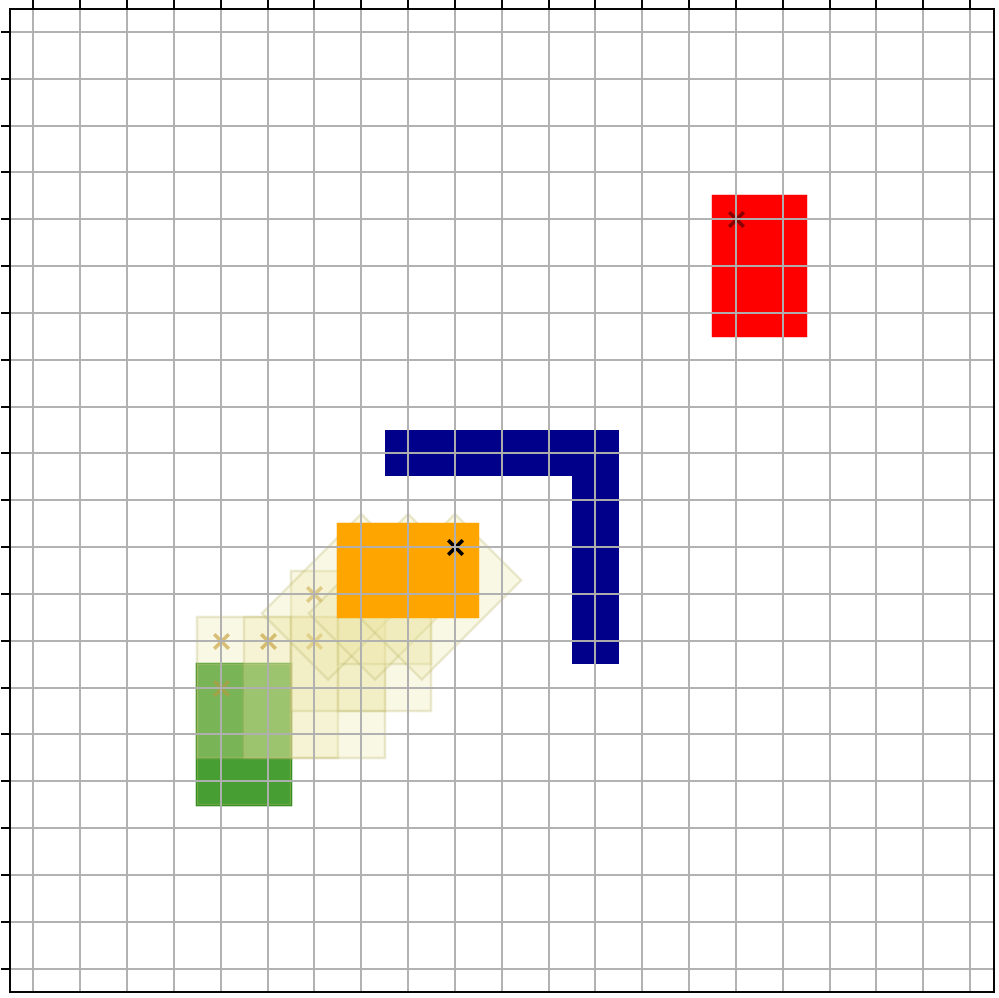
\includegraphics{bilder/attr-repul-c-shape.png}}}
	\caption{Für konkave Hindernisse in Potenzialfeldern berechnet mit anziehendem und abstoßendem Potenzial konvergiert das Gradientenabstiegsverfahren zu einem lokalen Minimum.}
\end{figure}

Weiterhin sind im Kraftfeld von Potenzialfeldern berechnet mit anziehendem und abstoßendem Potenzial zwischen Hindernisengstellen Oszillationen möglich. Der Roboter wechselt bei dieser Art des lokalen Minimums zwischen zwei Koordinaten mit entgegengerichteten Gradienten.
Insbesondere kleine Occupancy Grids sind von diesem Effekt betroffen, da die X- und Y-Grenzen als Hindernisse interpretiert werden. Abbildung \ref{fig:oscillation} zeigt diesen Effekt anhand des Potenzialfelds aus Kapitel \ref{sec:attr-repul-pot}.
Die Erhöhung des Abstandes zwischen den Grenzen des Occupancy-Grid und Hindernissen vermeidet dieses Problem.
\begin{figure}[H]
	\footnotesize
	\centering
	\hspace*{\fill}
	\begin{minipage}{0.46\textwidth}%
		\centerline{\resizebox{0.65\linewidth}{!}{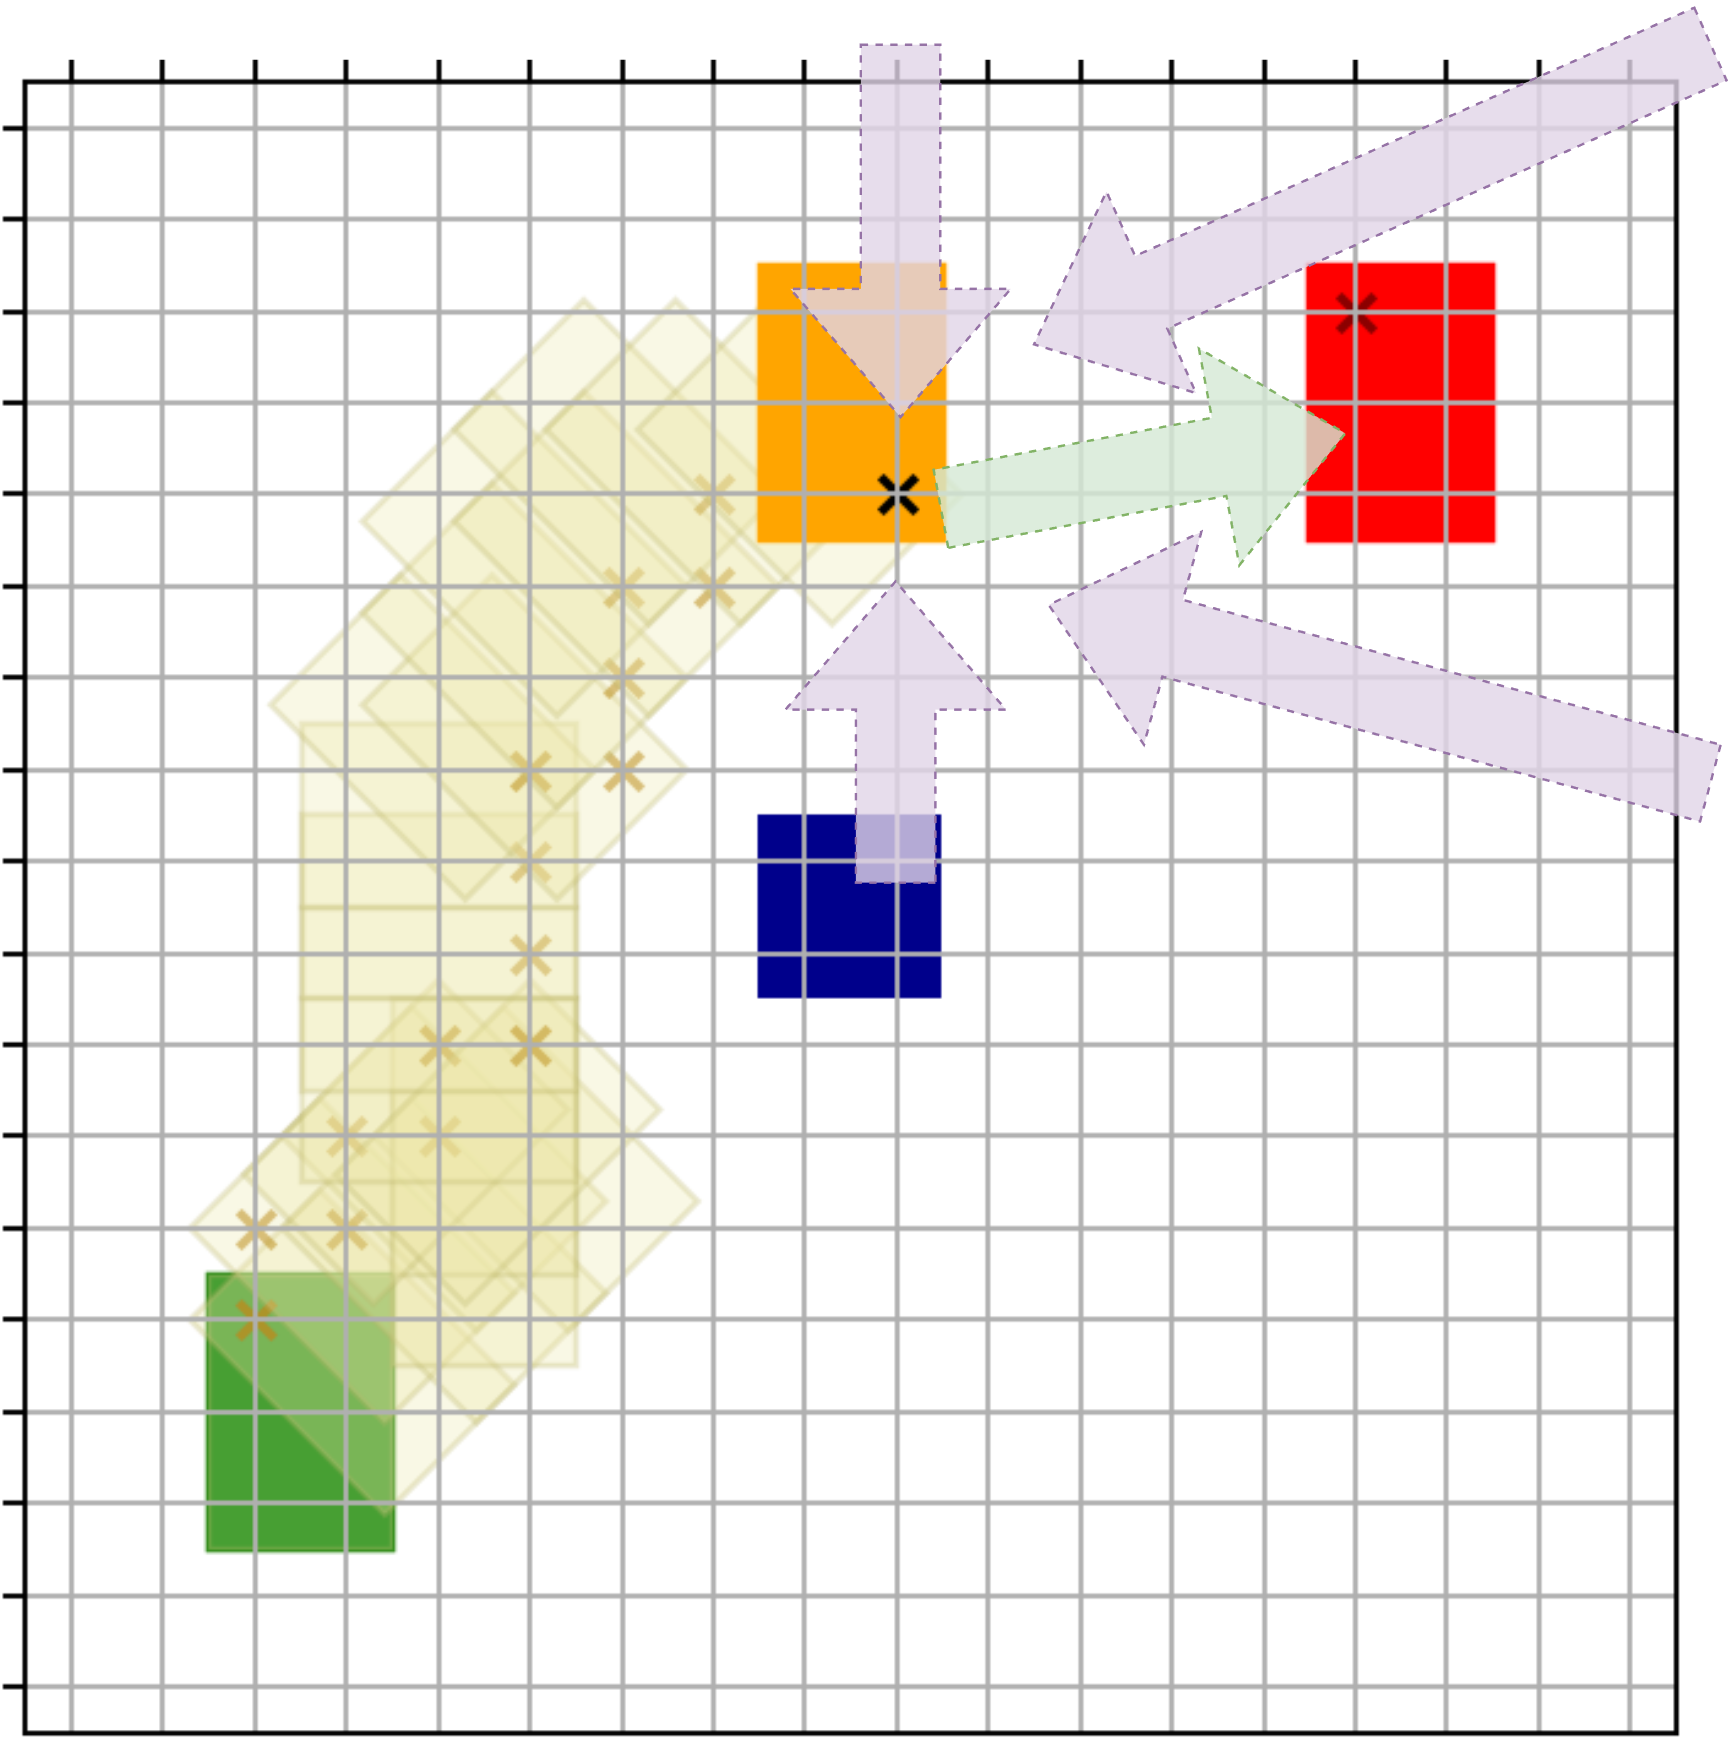
\includegraphics{bilder/attr-repul-oscillating-arrow.png}}}
	\end{minipage}
	\hspace*{\fill}
	\begin{minipage}{0.46\textwidth}%
		\footnotesize
		\centerline{\resizebox{0.65\linewidth}{!}{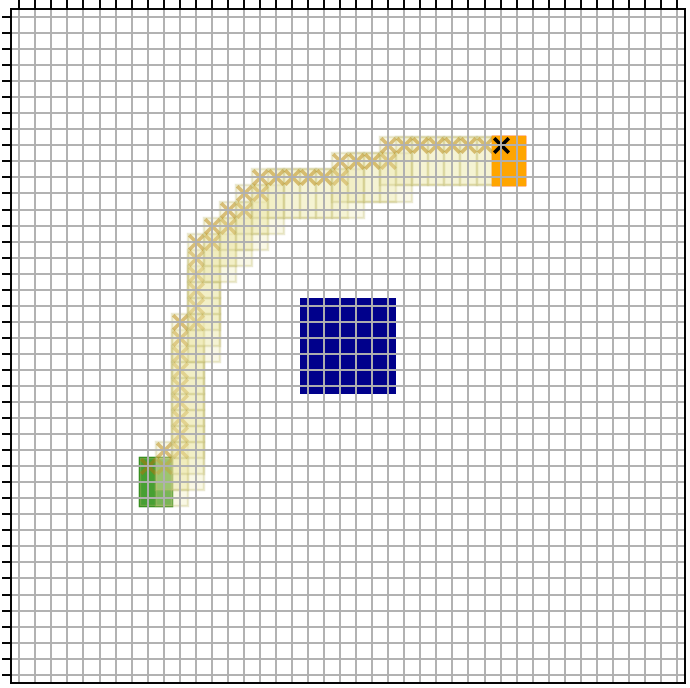
\includegraphics{bilder/attr-repul-oscillating-scaled.png}}}
	\end{minipage}
	\hspace*{\fill}
	%	\vspace{-1cm}
	\label{fig:oscillation}
	\caption{Bei Engstellen oszillieren die abstoßenden Kräfte zwischen Hindernissen (links), bei hinreichend Abstand nicht (rechts).}
\end{figure}

Im Gegensatz dazu verhindert die streng monotone Potenzialänderung des Wavefront-Algorithmus die Konvergenz zu lokalen Minima, sofern sich das Ziel an einem für den Roboter physikalisch erreichbaren Punkt befindet.
\vspace*{0.1cm}
\begin{figure}[H]
	\footnotesize
	\centering
	\centerline{\resizebox{1\linewidth}{!}{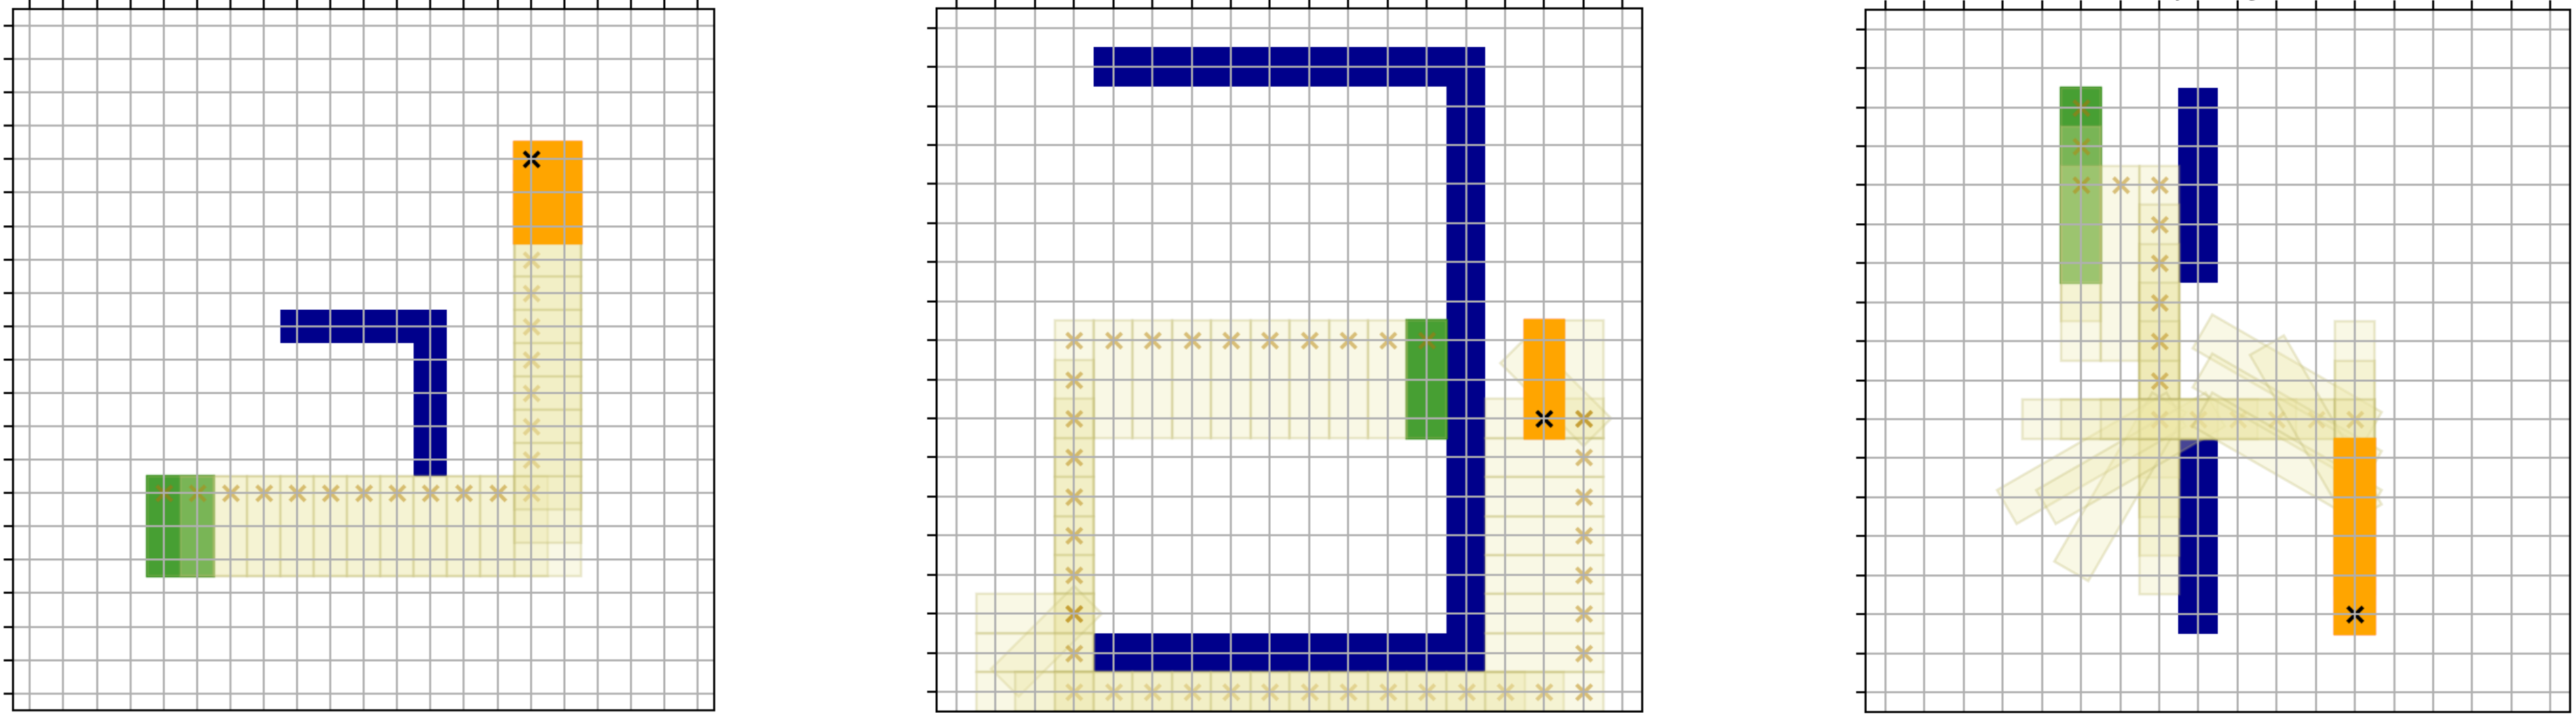
\includegraphics{bilder/wavefront-demo.png}}}
	\caption{Das Gradientenabstiegsverfahren in Kraftfeldern der Wavefront-Potenzialfelder konvergiert zum Zielpunkt.}
\end{figure}

\vspace*{0.1cm}
\section{Interpolationsartefakte}

Wie in Kapitel \ref{ch:config-space} beschrieben, wird bei der Berechnung des Konfigurationsraums die Roboterrotation in \texttt{rotation\_step}s diskretisiert. Dazu wird für das Robotermodell eine Array-Maske über die Matrixrotation \texttt{sklearn.rotate()} gedreht. 

Insbesondere bei kleinen Roboterdimensionen mit kleinen Rotationswinkeln entstehen hier \textit{Interpolationsartefakte}.
Dies zeigt sich bei der Visualisierung der Roboternavigation durch die Überdeckung von Hindernissen mit dem Robotermodell. Yunfeng und Chirikjian empfehlen deshalb, für kleine Rotationswinkel die Roboterdimensionen sowie das Occupancy Grid zu skalieren \cite{yujiang.2017}.
Somit wird die Auflösung der Robotermaske erhöht und die Artefakte der Interpolation verringert.
\vspace*{0.5cm}
\begin{figure}[h!]
	\footnotesize
	\centering
	\hspace*{-0.1\linewidth}
	\centerline{\resizebox{1.2\linewidth}{!}{
	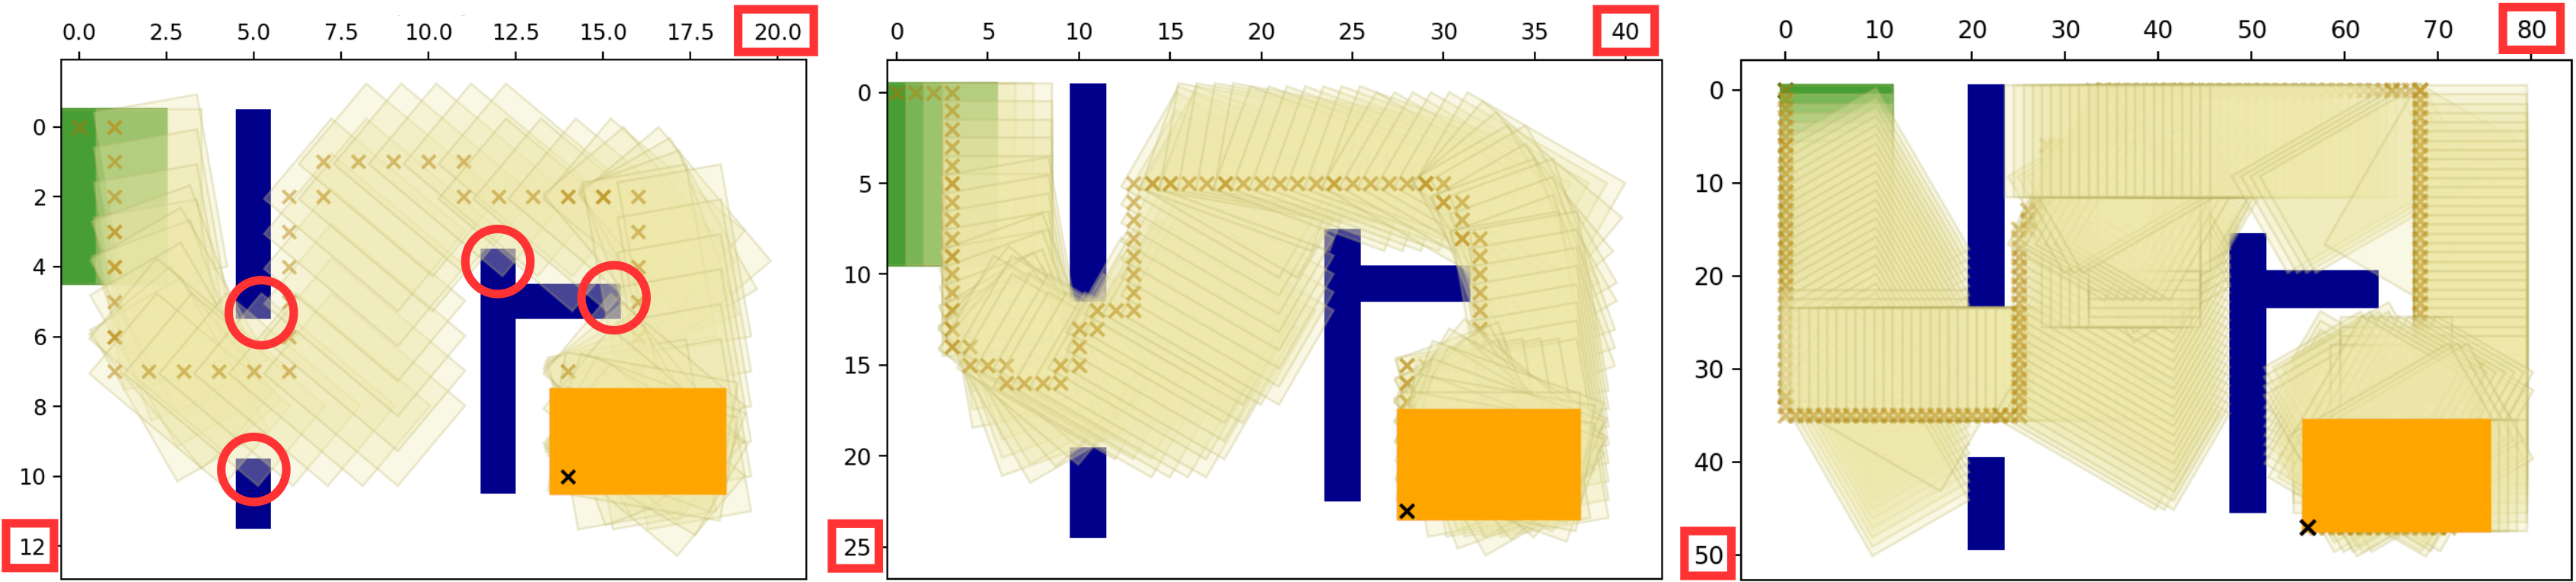
\includegraphics{bilder/occu-scaling6.png}
	}}
	\hspace*{-0.1\linewidth}
	\vspace*{0.3cm}
	\caption{Die sukzessive Verdopplung der Dimensionen des Robotermodells und Occupancy Grids verringert die Interpolationsartefakte.}
\end{figure}







